%Version 3 October 2023


%%\documentclass[referee,sn-basic]{sn-jnl}% referee option is meant for double line spacing

%%=======================================================%%
%% to print line numbers in the margin use lineno option %%
%%=======================================================%%

%%\documentclass[lineno,sn-basic]{sn-jnl}% Basic Springer Nature Reference Style/Chemistry Reference Style

%%======================================================%%
%% to compile with pdflatex/xelatex use pdflatex option %%
%%======================================================%%

%%=============================================================%%
%% GivenName	-> \fnm{Joergen W.}
%% Particle	-> \spfx{van der} -> surname prefix
%% FamilyName	-> \sur{Ploeg}
%% Suffix	-> \sfx{IV}
%% \author*[1,2]{\fnm{Joergen W.} \spfx{van der} \sur{Ploeg} 
%%  \sfx{IV}}\email{iauthor@gmail.com}
%%=============================================================%%


%%==================================%%
%% Sample for unstructured abstract %%%\author*[1,2]{\fnm{First} \sur{Author}}\email{iauthor@gmail.com}
%
%\author[2,3]{\fnm{Second} \sur{Author}}\email{iiauthor@gmail.com}
%\equalcont{These authors contributed equally to this work.}
%
%\author[1,2]{\fnm{Third} \sur{Author}}\email{iiiauthor@gmail.com}
%\equalcont{These authors contributed equally to this work.}
%
%\affil*[1]{\orgdiv{Department}, \orgname{Organization}, \orgaddress{\street{Street}, \city{City}, \postcode{100190}, \state{State}, \country{Country}}}
%%==================================%%

%\abstract{The abstract serves both as a general introduction to the topic and as a brief, non-technical summary of the main results and their implications. Authors are advised to check the author instructions for the journal they are submitting to for word limits and if structural elements like subheadings, citations, or equations are permitted.}

%%================================%%
%% Sample for structured abstract %%
%%================================%%

% \abstract{\textbf{Purpose:} 
% 
% \textbf{Methods:}
% 
% \textbf{Results:} 
% 
% \textbf{Conclusion:} }

%\keywords{keyword1, Keyword2, Keyword3, Keyword4}

%%\pacs[JEL Classification]{D8, H51}

%%\pacs[MSC Classification]{35A01, 65L10, 65L12, 65L20, 65L70}

% Reference Style/Chemistry Reference Style


%%\documentclass[sn-nature]{sn-jnl}% Style for submissions to Nature Portfolio journals
%%\documentclass[sn-basic]{sn-jnl}% Basic Springer Nature Reference Style/Chemistry Reference Style
%%\documentclass[sn-mathphys-num]{sn-jnl}% Math and Physical Sciences Numbered Reference Style 
%%\documentclass[sn-mathphys-ay]{sn-jnl}% Math and Physical Sciences Author Year Reference Style
%%\documentclass[sn-aps]{sn-jnl}% American Physical Society (APS) Reference Style
%%\documentclass[sn-vancouver,Numbered]{sn-jnl}% Vancouver Reference Style
%%\documentclass[sn-apa]{sn-jnl}% APA Reference Style 
%%\documentclass[sn-chicago]{sn-jnl}% Chicago-based Humanities Reference Style

%%%% Standard Packages
%%<additional latex packages if required can be included here>



%%%%%=============================================================================%%%%
%%%%  Remarks: This template is provided to aid authors with the preparation
%%%%  of original research articles intended for submission to journals published 
%%%%  by Springer Nature. The guidance has been prepared in partnership with 
%%%%  production teams to conform to Springer Nature technical requirements. 
%%%%  Editorial and presentation requirements differ among journal portfolios and 
%%%%  research disciplines. You may find sections in this template are irrelevant 
%%%%  to your work and are empowered to omit any such section if allowed by the 
%%%%  journal you intend to submit to. The submission guidelines and policies 
%%%%  of the journal take precedence. A detailed User Manual is available in the 
%%%%  template package for technical guidance.
%%%%%=============================================================================%%%%

\documentclass[pdflatex,sn-mathphys-num]{sn-jnl}% Basic Springer Nature
\usepackage{multirow}%
\usepackage{graphicx}
\usepackage{amsmath,amssymb,amsfonts}%
\usepackage{amsthm}%
\usepackage{mathrsfs}%
\usepackage[title]{appendix}%
\usepackage[dvipdfmx]{xcolor}%
\usepackage{textcomp}%
\usepackage{manyfoot}%
\usepackage{booktabs}%
\usepackage{algorithm}%
\usepackage{algorithmicx}%
\usepackage{algpseudocode}%
\usepackage{listings}%
\usepackage[xindy]{glossaries}
\usepackage{ulem}
\usepackage{bm}
\usepackage{caption}
\captionsetup[table]{justification=centering}
\captionsetup[figure]{justification=centering}
\renewcommand{\glossarysection}[2][]{}

%% as per the requirement new theorem styles can be included as shown below
\theoremstyle{thmstyleone}%
\newtheorem{theorem}{Theorem}%  meant for continuous numbers
%%\newtheorem{theorem}{Theorem}[section]% meant for sectionwise numbers
%% optional argument [theorem] produces theorem numbering sequence instead of independent numbers for Proposition
\newtheorem{proposition}[theorem]{Proposition}% 
%%\newtheorem{proposition}{Proposition}% to get separate numbers for theorem and proposition etc.

\theoremstyle{thmstyletwo}%
\newtheorem{example}{Example}%
\newtheorem{remark}{Remark}%

\theoremstyle{thmstylethree}%
\newtheorem{definition}{Definition}%
\makeglossaries
\setacronymstyle{long-short-desc}
\loadglsentries{glossary.tex}
\newcommand{\pname}[1]{``{\uline{\sl {#1}}}''}
\newcommand{\mainpname}[1]{``{\sl {#1}}''}
\newcommand{\inprep}{
	\begin{center}
		\sl\rm {!!!!In preparation!!!!}
\end{center}}

%%%%
\raggedbottom

%%\unnumbered% uncomment this for unnumbered level heads
\begin{document}
	\title[Basic theory behind (X)PBD]{Basic theory behind (X)PBD}
	\author*{\fnm{Slime} \sur{Piki}(Taisei Kunimi)}
\maketitle
\tableofcontents
\newpage

\section{Introduction}\label{sec1}
\subsection{What is (X)PBD?}
PBD is one of the simulation theories that basically simulates \gls{softBody} or \gls{elasticBody}.

PBD (Position Based Dynamics) proposed at \cite{PBD} is a popular method because of its stability and ease of implementation.In datail, PBD computes physical simulation only using positions inside the \gls{iteration}s and all we have to do is compute displacement and modify them.
In other words, we don't have to use complicated numerical analysis theories, it sounds pretty good.

But, in contrast to ease of implementation, it isn't easy to understand PBD's background theory. This is the problem when modifying PBD depending on your purpose. 

If you start your research from the original PBD paper\cite{PBD}, you will wonder how the authors derive constraints' formulations or why this solver works well. Or you start from XPBD \cite{XPBD}, you will be confused by the suddenly appeared Lagrange multiplier or energy potential that we don't know how to handle.
Unfortunately, we can't know much from them and it may be common in literature search, there is no clear path to learning them. Then, I decided to write a guidebook on the underlying theory of PBD.

\subsection{Difference from existing PBD coursenote}
Actually, there are some course notes on PBD written by authors who published papers on PBD and XPBD, e.g. \cite{PBDCoursenote}. These course notes describe the basic style of PBD and its extensions. But there is the same problem we saw in \cite{PBD} and \cite{XPBD}, that is, how to implement is described but why this method works well is not. Thus, I believe that this document isn't meaningless. Well then, let's start the journey to XPBD!

\subsection{Learning Path}
Fig. \ref{XPBDPath} shows the shortest path to understand (X)PBD. You don't have to read this note from head to tail because this note covers wide topics around (X)PBD. If you only want to learn how (X)PBD works, you read this note along with Fig. \ref{XPBDPath}'s path. In addition, the dashed circles could be skipped if you are in a hurry.

\begin{figure}[h]
	\centering
	\begin{minipage}[b]{0.49\columnwidth}
	\centering
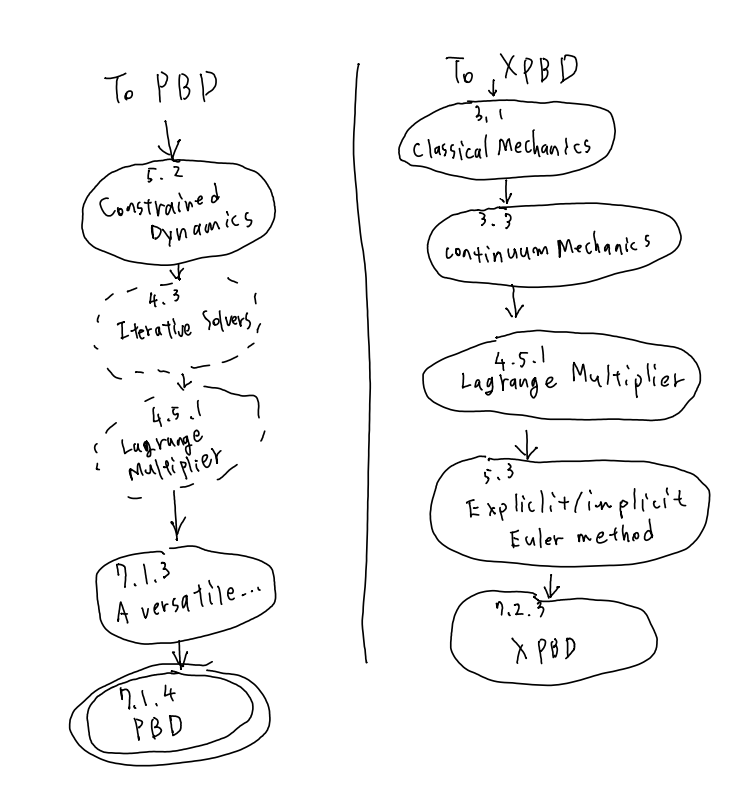
\includegraphics[width=1.05\textwidth]{images/(X)PBD_path.png}
\caption{Path to (X)PBD}
\label{XPBDPath}
	\end{minipage}
	\begin{minipage}[b]{0.49\columnwidth}
	\centering
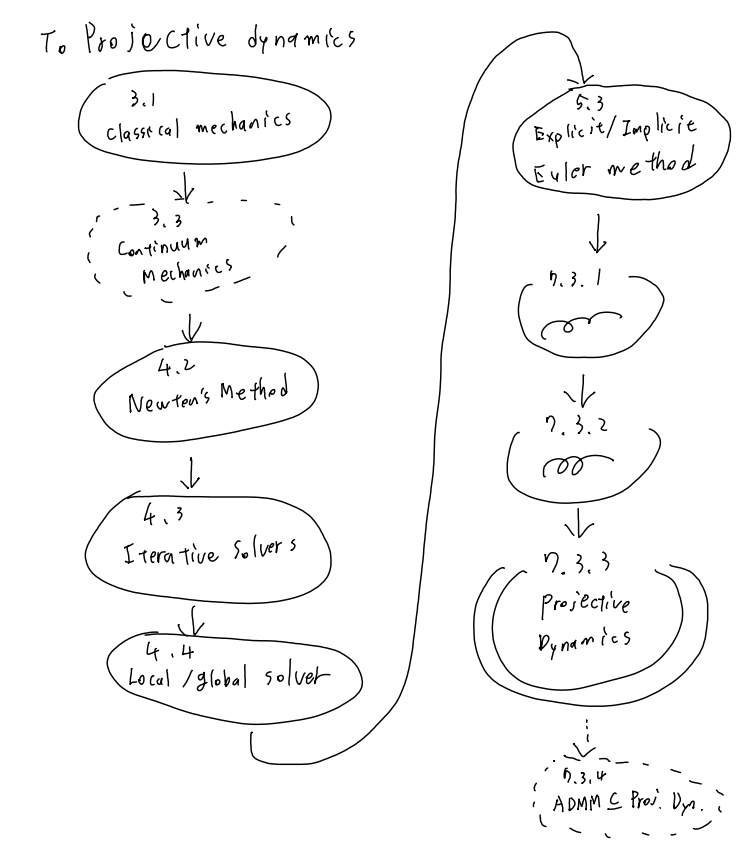
\includegraphics[width=1.1\textwidth]{images/ProjDyn_path.png}
\caption{Path to (X)PBD}
\label{ProjPath}
	\end{minipage}
\end{figure}

As the extra, you can use this note to learn Projective Dynamics also, yay!
If you want to do so, the shortest path is fig. \ref{ProjPath}.

\section{The history of PBD}
I think starting from history is a good way to learn something because there are no leaps in logic and it will be easy to understand where we are. However, there is certainly redundancy, so you can skip this section to save time. I'll make an effort to write that you can understand everything even if you skipped this section.

The history of PBD can be roughly divided into three parts.
Let them are pre-PBD, post-PBD and post-XPBD.

\subsection{Pre-PBD}
\begin{figure}[h]
\centering
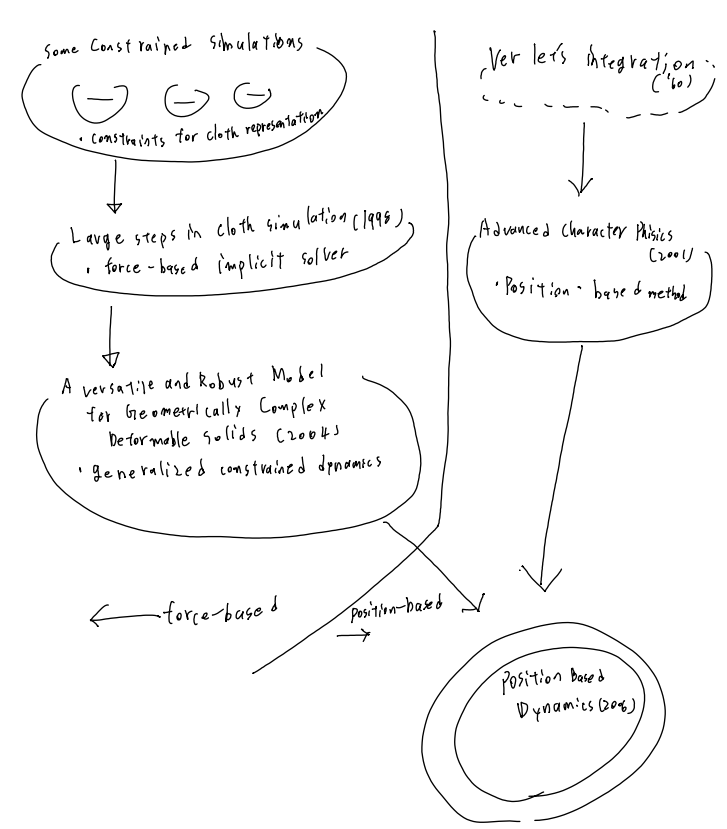
\includegraphics[width=0.8\textwidth]{images/prePBD.png}
\caption{history of pre-PBD}
\label{prePBD}
\end{figure}

The flow of the pre-PBD began from the appearance of constraint dynamics(\cite{EnergyWitkin1987}, \cite{ConstrainedBarzel} and \cite{ConstrainedPlatt}) through \mainpname{Large Steps in Cloth Simulation}\cite{LargeStepBaraff} used \gls{constraint}s as shape representation and simulates cloth with energy form \gls{constraint}s' gradients, \mainpname{Advanced Character Physics}\cite{Jakobsen2003AdvancedCP} introduces position-based approach derived from Verlet's integration scheme with the distance constraints and \mainpname{A Versatile and Robust Model for Geometrically Complex Deformable Solids}\cite{VersatileTeschner} generalize \cite{LargeStepBaraff}'s method.
And, finally, \mainpname{Position Based Dynamics}\cite{PBD} introduced the generalized constraints method from \cite{VersatileTeschner} into \cite{Jakobsen2003AdvancedCP}'s position-based simulation to use various \gls{constraint}s.

\subsection{Post-PBD}
\begin{figure}[h]
	\centering
	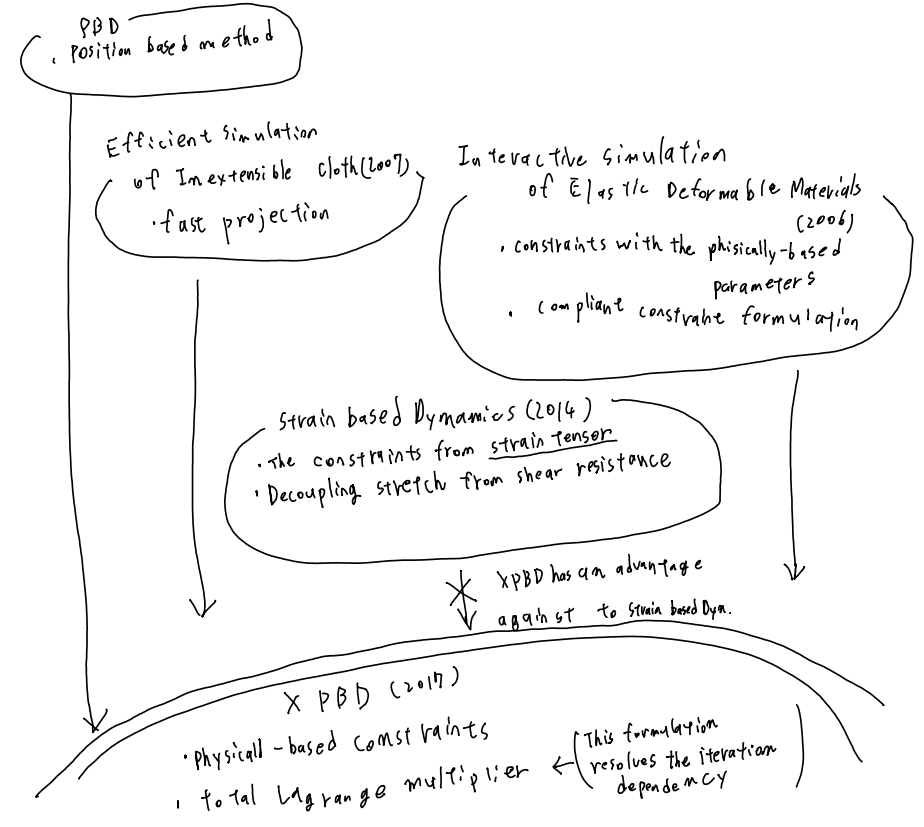
\includegraphics[width=1\textwidth]{images/postPBD.png}
	\caption{history of post-PBD}
		\label{postPBD}
\end{figure}

From the published PBD paper, a lot of study about it has been done.
The central development is resolving well-known PBD's drawback whose result depends on \gls{iteration} times, at \mainpname{XPBD: position-based simulation of compliant constrained dynamics}\cite{XPBD}.

To understand XPBD, we need some knowledge of continuum mechanics.
The theory directly used in XPBD is derived from \mainpname{Interactive simulation of elastic deformable materials}\cite{Servin2006InteractiveSO} that uses the theory for \gls{LagrangianMechanics}.

Besides that, some papers also influence XPBD, \mainpname{Efficient simulation of inextensible cloth}\cite{EfficientGoldenthai} and \mainpname{Strain Based Dynamics}\cite{StrainBasedDyn} are examples of them.
The former introduces the projection method described later. The latter invites physically based constraints to PBD.

Although there is relevance to XPBD, the key idea to construct XPBD is \cite{Servin2006InteractiveSO} and aren't the last two papers. In other words, to understand XPBD, we truly only have to read \cite{Servin2006InteractiveSO} or get the equivalent knowledge.

But, unfortunately, the key idea of XPBD provided by \cite{Servin2006InteractiveSO} doesn't have a sufficient explanation of where the authors get the formulation. Then, I guess a description later that seemed reasonable enough.

\subsection{Post-XPBD}
Shortly after published XPBD paper, a simple but important improvement was provided at \mainpname{Small steps in physics simulation}\cite{SmallSteps}.
\inprep
\section{Physics}
This section is devoted to fundamental physics. 

Of course, the physics simulation field takes advantage of the basics.
If we only handle trivial environments, classical mechanics can achieve simulation. 

However, classical mechanics isn't enough to simulate complex objects or get plausible results. For example, Newtonian mechanics-based methods suffer from soft-body simulation, and so on.

The algorithm of the soft-body simulation isn't trivial, and there is no definitive solution at present. Therefore, many methods have been studied to solve this problem.

Based on the above perspective, in this section, I also introduce some physical theories that are frequently used in soft/elastic body simulation, Constrained dynamics, and Continuum mechanics.
In particular, continuum mechanics is vital to understanding XPBD.
\begin{figure}[h]
	\centering
	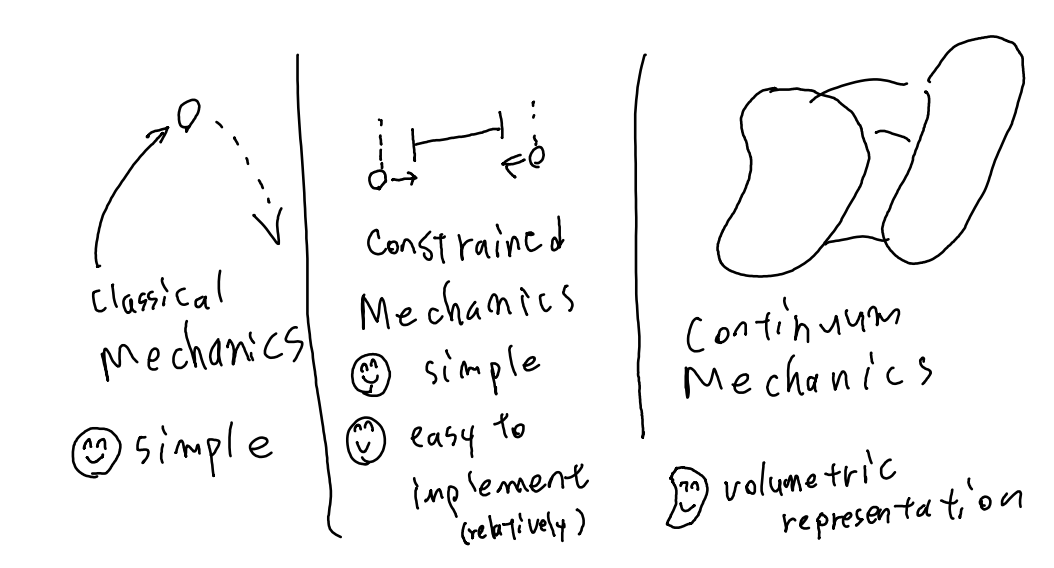
\includegraphics[width=0.8\textwidth]{images/Physics.png}
	\caption{Comparison of the physics}
		\label{physics}
\end{figure}

Although there are many other important theories, such as fluid mechanics or thermodynamics, I won't explain them because this document's subject is (X)PBD which focuses on soft/elastic body (actually, PBD can be used in fluid simulation...).

\subsection{Classical mechanics}
Let's start the physics course with classical mechanics.

First, please imagine a car running at a constant speed.
\inprep

\subsection{Constrained Dynamics}
\inprep
\subsection{Continuum mechanics}
\inprep
\subsubsection{What is tensor?}
\inprep
\subsubsection{Force, strain, and stress}
\inprep
\subsubsection{Kirchhoff stress tensor}
\inprep
\subsubsection{Cauchy-Green deformation tensor}
\inprep
\subsubsection{St. Venant strain tensor}
\inprep

\section{Numerical integration}
\inprep
\subsection{The linear solvers}
\inprep
\subsection{Newton's method}
\inprep
\subsection{Iterative solvers}
\inprep
\subsection{Local/global solver}
\inprep
\subsection{Misc. topics}
\inprep
\subsubsection{Lagrange Multiplier}
\inprep
\subsubsection{LU decomposition}
\inprep
\subsubsection{Schur decomposition}
\inprep

\section{Numerical physics}
\inprep
\subsection{Verlet's integration}
\inprep
\subsection{Mass-spring system}
\inprep
\subsection{Explicit/implicit Euler method}
\inprep
\subsection{Shape matching}
\inprep

\section{Column : In the terminology mess}
\inprep
\subsection{Newton*}
\inprep
\subsection{Euler*}
\inprep
\subsection{Jacobi*}
\inprep
\subsection{Lagrange*, Hamilton*, Hesse*}
\inprep

\section{Interplet the papers}
\inprep
\subsection{To PBD}
\inprep
\subsubsection{{\sl Large steps in cloth simulation}\cite{LargeStepBaraff}}
\inprep
\subsubsection{{\sl Advanced Character Physics}\cite{Jakobsen2003AdvancedCP}}
\inprep
\subsubsection{\small{\sl A Versatile and Robust Model for Geometrically Complex Deformable Solids}\cite{VersatileTeschner}}
\inprep
\subsubsection{{\sl Position Based Dynamics}\cite{PBD}}
\inprep

\subsection{To XPBD}
\inprep
\subsubsection{{\sl Geometric, Variational Integrators for Computer Animation}\cite{VariationalIntegrators2006}}
\inprep
\subsubsection{{\sl Interactive simulation of elastic deformable materials}\cite{Servin2006InteractiveSO}}
\inprep
\subsubsection{\small{\sl XPBD : position-based simulation of compliant constrained dynamics}\cite{XPBD}}
\inprep

\subsubsection{{\sl Small steps in physics simulation}\cite{SmallSteps}}
\inprep
\subsection{Bonus section : Projective Dynamics}
\inprep
\subsubsection{{\sl Example-based elastic materials}\cite{Example-basedMartin}}
\inprep
\subsubsection{{\sl Fast simulation of mass-spring systems}\cite{fastMassTiantian}}
\inprep
\subsubsection{\small{\sl Projective Dynamics: Fusing Constraint Projections for Fast Simulation}\cite{ProjDyn}}
\inprep
\subsubsection{\small{\sl ADMM $\subseteq$ projective dynamics: fast simulation of general constitutive models}\cite{ADMM_Proj}}
\inprep

\subsection{Post-XPBD}
\inprep
\newpage
\appendix




\section{Inportance of papers}
A lower number means more important. The papers' names are aligned in the lexicographic order as possible as I can.
\begin{enumerate}
	\item You must read these papers if you want to understand (X)PBD. But if you want to understand them completely, I recommend reading the others also.
		\begin{itemize}
			\item \pname{Position Based Dynamics}\cite{PBD} is one of the main subjects of this document.
			\newline
			\item \pname{XPBD : position-based simulation of compliant constrained dynamics}\cite{XPBD} addressed a numerical artifact that makes dependency between stiffness and \gls{iteration} count or size of the time-step.
		\end{itemize}
		\item  These papers are vital in understanding (X)PBD or have a strong impact on the field.
		\begin{itemize}
			\item\pname{Advanced Character Physics}\cite{Jakobsen2003AdvancedCP} introduced position based simulation method derived from Verlet's integration scheme and combined distance constraints. The framework of PBD can be seen here. Specifically,using distance and angular constraints, modifying verticies' position directoly and solving \gls{constraint}s with some iterations. This paper is easier to read than PBD, but the ideas appear here and pseudo codes are presented. I recommend reading this before read PBD.
			\newline
			\item \pname{Large steps in cloth simulation}\cite{LargeStepBaraff} solved implicit integration with \gls{constraint}s by \gls{cgmethod} for off-line simulation. The scheme isn't used at PBD, but this one gives us a perspective of present physical simulations.
			\newline
			\item \pname{Projective Dynamics: Fusing Constraint Projections for Fast Simulation}\cite{ProjDyn} provided a position-based method that uses energy formulation and local/global solver. The method has a local Jacobi-like solver and a linear global equation one. The solvers enable robust and fast simulation without safeguards against singular or indefinite Hessians.
			If you want to understand state-of-the-art physics simulation methods, including PBD, it's better to read this.
			\newline
			\item \pname{ADMM $\subseteq$ projective dynamics: fast simulation of general constitutive models}\cite{ADMM_Proj} is worth reading because ADMM is actively researched now because of its robustness, parallelizability, and simplicity. 
		\end{itemize}
		\item These papers offer interesting discussions around PBD, deepen your understanding of PBD, or description of basic physical simulation scheme.
		\begin{itemize}
			\item \pname{Constraint Methods for Neural Networks and Computer Graphics}\cite{ConstrainedPlatt} describes the constraint methods for neural networks and computer graphics.
			It may not be easy to read because of 150 pages. But, if you have time, it's more worth reading this paper than some papers published before this one.
			\newline
			\item \pname{Example-based elastic materials}\cite{Example-basedMartin} provides a concept of the elastic manifold and optimization method for deforming into an artist-desirable state. However, this paper lacks reference to the manifold projection methods that are apparently well-known in the geometric optimization field.This paper helps us understand Projective dynamics, but I don't know Projective Dynamics's relevance with (X)PBD for now.
			\newline
			\item \pname{Fast simulation of mass-spring systems}\cite{fastMassTiantian} describes the local/global type solver to the mass-spring system clearly. Thus this paper helps us understand the variant solvers.
			\newline
			\item \pname{Interactive simulation of elastic deformable materials}\cite{Servin2006InteractiveSO} introduces physical parameters into constrained dynamics; the spirit is inherited by XPBD and there is an interesting discussion about the integrator. But I think this paper does explain the concept poorly,e. g. the integrator provided here, equation (20) lack of explanation, etc. 
			Therefore, this one classified here.
			\newline
			\item \pname{Nucleus: Towards a unified dynamics solver for computer graphics}\cite{Nucleus} is a good introduction to constrained dynamics because it shows its implementation aspect.
			However, it doesn't describe how constraints are resolved, so it isn't full-contained.
			\newline
			\item \pname{Robust treatment of collisions, contact and friction for cloth animation}\cite{RobustBridson2002}'s scheme separates physical simulation into internal parts and external parts. 
			Therefore, we can choose the internal modeling(e.g. mass-spring) and the external modeling(e.g. collision repulsion, friction, or gravity) independently. However, the scheme is not directly related to PBD.
			\newline
			\item \pname{Strain Based Dynamics}\cite{StrainBasedDyn}. The formulation of the strain tensor in XPBD seems to be based on 
			"Interactive Simulation of Elastic Deformable Materials"(2006) rather than this paper.
			However, the formulations described here are easy to understand if you are familiar with PBD and strain tensor.
			\newline
			\item \pname{Geometric, Variational Integrators for Computer Animation}\cite{VariationalIntegrators2006} presents the variational integrator from the Lagrangian/Hamiltonian physics that preserves linear/angular momenta.
			Its conservative quantities will be more important in fields such as robotics or accurate physical computation.
			But, this knowledge may be useless if you only want to understand  (X)PBD.
			\newline
			\item \pname{Efficient simulation of inextensible cloth}\cite{EfficientGoldenthai} treated the constrained system as globally linearized form and solved with a direct approach at each iteration.
		\end{itemize}
	\item These ones have historical value, but deeper discussions are done in other papers.
		\begin{itemize}
		\item \pname{Elastically deformable models}\cite{ElasticTerzopoulos}  brought the formulation of elastic bodies to computer graphics.
		\newline
		\item \pname{Energy Constraints On Parameterized Models}\cite{Witkin1987} uses shape representations that quite different from the current ones and the constraints presented in this paper are slightly inconvenient to the current ones. Thus, we no longer have to read this.
		\newline
		\item \pname{A modeling system based on dynamic constraints}\cite{Barzel1988} uses constraints as models' motion rather than to hold a model's detail and uses linear simultaneous equations when deriving forces.The points that are difficult to understand are that the paper doesn't describe the background of the equation derivation and that the symbols are scattered too much.
		Fortunately, we don't have to read this paper completely to understand present constrained dynamics because the style varies from the recent ones.
		\end{itemize}
	\item Not be classified yet.
		\begin{itemize}
			\item \pname{A Versatile and Robust Model for Geometrically Complex Deformable Solids}\cite{VersatileTeschner}
			\item \pname{Meshless deformations based on shape matching}\cite{MeshlessMuller2005}
			\item \pname{Fast Simulation of Inextensible Hair and Fur}\cite{InextensibleHair}
			\item \pname{Long Range Attachments - A Method to Simulate Inextensible Clothing in Computer Games}\cite{LongRangeAttachments}
			\item \pname{Position Based Fluids}\cite{PosBaseFluids}
			\item \pname{Position-based simulation of continuous materials}\cite{PBContimuousBENDER2014}
			\item \pname{Unified particle physics for real-time applications}\cite{UnifiedParticle}
			\item \pname{Air Meshes for Robust Collision Handling}\cite{AirMesh}
			\item \pname{A survey on position based dynamics, 2017}\cite{PBDCoursenote}
			\item \pname{Stable Constrained Dynamics}\cite{StableConstrainedDyn}
			\item \pname{Small steps in physics simulation}\cite{SmallSteps}
			\item \pname{Non-Smooth Newton Methods for Deformable Multi-Body Dynamics}\cite{NonSmooth}
			\item \pname{Detailed Rigid Body Simulation with Extended Position Based Dynamics}\cite{DetailedRigidbody}
			\item \pname{A Constraint-based Formulation of Stable Neo-Hookean Materials}\cite{ConstrainedBasedNeo-Hookean}
			\item \pname{Physically Based Shape Matching}\cite{PhysBaseShapeMatching}
			\item \pname{}\cite{}
			\item \pname{}\cite{}
			\item \pname{}\cite{}
			\item \pname{}\cite{}
			\item \pname{}\cite{}
			\item \pname{}\cite{}
			\item \pname{}\cite{}
			\item \pname{}\cite{}
			\item \pname{}\cite{}
			\item \pname{}\cite{}
			\item \pname{}\cite{}
			\item \pname{}\cite{}
			\item \pname{}\cite{}
			\item \pname{}\cite{}
			\item \pname{}\cite{}
			\item \pname{}\cite{}
			\item \pname{}\cite{}
			\item \pname{}\cite{}
			\item \pname{}\cite{}
			\item \pname{}\cite{}
			\item \pname{}\cite{}
			\item \pname{}\cite{}
			\item \pname{}\cite{}
			\item \pname{}\cite{}
		\end{itemize}
	
\end{enumerate}


\section{Glossaly}\label{ap1}
\subsection{symbols}

\subsection{terms}
\printglossary[nonumberlist, title={\hspace{-30pt}}, style=altlist]

\appendix

\addcontentsline{toc}{section}{References}
\bibliography{sn-bibliography}% common bib file


\end{document}


% \cite{bib1} 

%%==================%%
%% equation samples %%
%%==================%%
%\section{Equations}\label{sec4}
%$H\psi = E \psi$ is written via the command \verb+$H \psi = E \psi$+.

%\begin{equation}
%\|\tilde{X}(k)\|^2 \leq\frac{\sum\limits_{i=1}^{p}\left\|\tilde{Y}_i(k)\right\|^2+\sum\limits_{j=1}^{q}\left\|\tilde{Z}_j(k)\right\|^2 }{p+q}.\label{eq1}
%\end{equation}

%where,

%\begin{align}
%D_\mu &=  \partial_\mu - ig \frac{\lambda^a}{2} A^a_\mu \nonumber \\
%F^a_{\mu\nu} &= \partial_\mu A^a_\nu - \partial_\nu A^a_\mu + g f^{abc} A^b_\mu A^a_\nu \label{eq2}
%\end{align}

%\begin{equation}
%Y_\infty = \left( \frac{m}{\textrm{GeV}} \right)^{-3}
%    \left[ 1 + \frac{3 \ln(m/\textrm{GeV})}{15}
%    + \frac{\ln(c_2/5)}{15} \right]
%\end{equation}


%%==============%%
%%Table samples %%
%%==============%%

%\begin{table}[h]
%\caption{Caption text}\label{tab1}%
%\begin{tabular}{@{}llll@{}}
%\toprule
%Column 1 & Column 2  & Column 3 & Column 4\\
%\midrule
%row 1    & data 1   & data 2  & data 3  \\
%row 2    & data 4   & data 5\footnotemark[1]  & data 6  \\
%row 3    & data 7   & data 8  & data 9\footnotemark[2]  \\
%\botrule
%\end{tabular}
%\footnotetext{Source: This is an example of table footnote. This is an example of table footnote.}
%\footnotetext[1]{Example for a first table footnote. This is an example of table footnote.}
%\footnotetext[2]{Example for a second table footnote. This is an example of table footnote.}
%\end{table}

%===========================================================

%\begin{verbatim}
%\begin{table}[<placement-specifier>]
%\caption{<table-caption>}\label{<table-label>}%
%\begin{tabular}{@{}llll@{}}
%\toprule
%Column 1 & Column 2 & Column 3 & Column 4\\
%\midrule
%row 1 & data 1 & data 2	 & data 3 \\
%row 2 & data 4 & data 5\footnotemark[1] & data 6 \\
%row 3 & data 7 & data 8	 & data 9\footnotemark[2]\\
%\botrule
%\end{tabular}
%\footnotetext{Source: This is an example of table footnote. 
%This is an example of table footnote.}
%\footnotetext[1]{Example for a first table footnote.
%This is an example of table footnote.}
%\footnotetext[2]{Example for a second table footnote. 
%This is an example of table footnote.}
%\end{table}
%\end{verbatim}

%===========================================================

%\begin{table}[h]
%\caption{Example of a lengthy table which is set to full textwidth}\label{tab2}
%\begin{tabular*}{\textwidth}{@{\extracolsep\fill}lcccccc}
%\toprule%
%& \multicolumn{3}{@{}c@{}}{Element 1\footnotemark[1]} & \multicolumn{3}{@{}c@{}}{Element 2\footnotemark[2]} \\\cmidrule{2-4}\cmidrule{5-7}%
%Project & Energy & $\sigma_{calc}$ & $\sigma_{expt}$ & Energy & $\sigma_{calc}$ & $\sigma_{expt}$ \\
%\midrule
%Element 3  & 990 A & 1168 & $1547\pm12$ & 780 A & 1166 & $1239\pm100$\\
%Element 4  & 500 A & 961  & $922\pm10$  & 900 A & 1268 & $1092\pm40$\\
%\botrule
%\end{tabular*}
%\footnotetext{Note: This is an example of table footnote. This is an example of table footnote this is an example of table footnote this is an example of~table footnote this is an example of table footnote.}
%\footnotetext[1]{Example for a first table footnote.}
%\footnotetext[2]{Example for a second table footnote.}
%\end{table}

%===========================================================

%\begin{sidewaystable}
%\caption{Tables which are too long to fit, should be written using the ``sidewaystable'' environment as shown here}\label{tab3}
%\begin{tabular*}{\textheight}{@{\extracolsep\fill}lcccccc}
%\toprule%
%& \multicolumn{3}{@{}c@{}}{Element 1\footnotemark[1]}& \multicolumn{3}{@{}c@{}}{Element\footnotemark[2]} \\\cmidrule{2-4}\cmidrule{5-7}%
%Projectile & Energy	& $\sigma_{calc}$ & $\sigma_{expt}$ & Energy & $\sigma_{calc}$ & $\sigma_{expt}$ \\
%\midrule
%Element 3 & 990 A & 1168 & $1547\pm12$ & 780 A & 1166 & $1239\pm100$ \\
%Element 4 & 500 A & 961  & $922\pm10$  & 900 A & 1268 & $1092\pm40$ \\
%Element 5 & 990 A & 1168 & $1547\pm12$ & 780 A & 1166 & $1239\pm100$ \\
%Element 6 & 500 A & 961  & $922\pm10$  & 900 A & 1268 & $1092\pm40$ \\
%\botrule
%\end{tabular*}
%\footnotetext{Note: This is an example of table footnote this is an example of table footnote this is an example of table footnote this is an example of~table footnote this is an example of table footnote.}
%\footnotetext[1]{This is an example of table footnote.}
%\end{sidewaystable}


%%================%%
%%a figure sample %%
%%================%%
%\begin{figure}[h]
%\centering
%\includegraphics[width=0.9\textwidth]{fig.eps}
%\caption{This is a widefig. This is an example of long caption this is an example of long caption  this is an example of long caption this is an example of long caption}\label{fig1}
%\end{figure}


%%==============================================%%
%%Algorithms, Program codes and Listings samples%%
%%==============================================%%


%\lstset{texcl=true,basicstyle=\small\sf,commentstyle=\small\rm,mathescape=true,escapeinside={(*}{*)}}
%\begin{lstlisting}
%begin
%  for $i:=1$ to $10$ step $1$ do
%      expt($2,i$);  
%      newline() od                (*\textrm{Comments will be set flush to the right margin}*)
%where
%proc expt($x,n$) $\equiv$
%  $z:=1$;
%  do if $n=0$ then exit fi;
%     do if odd($n$) then exit fi;                 
%        comment: (*\textrm{This is a comment statement;}*)
%        $n:=n/2$; $x:=x*x$ od;
%     { $n>0$ };
%     $n:=n-1$; $z:=z*x$ od;
%  print($z$). 
%end
%\end{lstlisting}

%===========================================================

%
%\begin{algorithm}
%\caption{Calculate $y = x^n$}\label{algo1}
%\begin{algorithmic}[1]
%\Require $n \geq 0 \vee x \neq 0$
%\Ensure $y = x^n$ 
%\State $y \Leftarrow 1$
%\If{$n < 0$}\label{algln2}
%        \State $X \Leftarrow 1 / x$
%        \State $N \Leftarrow -n$
%\Else
%        \State $X \Leftarrow x$
%        \State $N \Leftarrow n$
%\EndIf
%\While{$N \neq 0$}
%        \If{$N$ is even}
%            \State $X \Leftarrow X \times X$
%            \State $N \Leftarrow N / 2$
%        \Else[$N$ is odd]
%            \State $y \Leftarrow y \times X$
%            \State $N \Leftarrow N - 1$
%        \EndIf
%\EndWhile
%\end{algorithmic}
%\end{algorithm}

%===========================================================

%\begin{minipage}{\hsize}%
%\lstset{frame=single,framexleftmargin=-1pt,framexrightmargin=-17pt,framesep=12pt,linewidth=0.98\textwidth,language=pascal}% Set your language (you can change the language for each code-block optionally)
%%%% Start your code-block
%\begin{lstlisting}
%for i:=maxint to 0 do
%begin
%{ do nothing }
%end;
%Write('Case insensitive ');
%Write('Pascal keywords.');
%\end{lstlisting}
%\end{minipage}

%%==================%%
%% citation samples %%
%%==================%%

%Here is an example for \verb+\cite{...}+: \cite{bib1}. Another example for \verb+\citep{...}+: \citep{bib2}. For author-year citation mode, \verb+\cite{...}+ prints Jones et al. (1990) and \verb+\citep{...}+ prints (Jones et al., 1990).

%===========================================================

%All cited bib entries are printed at the end of this article: \cite{bib3}, \cite{bib4}, \cite{bib5}, \cite{bib6}, \cite{bib7}, \cite{bib8}, \cite{bib9}, \cite{bib10}, \cite{bib11}, \cite{bib12} and \cite{bib13}.

%%====================%%
%% mathematic samples %%
%%====================%%

%\begin{tabular}{|l|p{19pc}|}
%\hline
%\verb+thmstyleone+ & Numbered, theorem head in bold font and theorem text in italic style \\\hline
%\verb+thmstyletwo+ & Numbered, theorem head in roman font and theorem text in italic style \\\hline
%\verb+thmstylethree+ & Numbered, theorem head in bold font and theorem text in roman style \\\hline
%\end{tabular}

%===========================================================

%\begin{theorem}[Theorem subhead]\label{thm1}
%\end{theorem}
%
%\begin{proposition}
%\end{proposition}
%
%\begin{example}
%\end{example}
%
%
%\begin{remark}
%\end{remark}
%
%\begin{definition}[Definition sub head]
%\end{definition}
%
%
%\begin{proof}
%\end{proof}
%
%
%\begin{proof}[Proof of Theorem~{\upshape\ref{thm1}}]
%\end{proof}
%
%\begin{quote}
%\end{quote}

 %(\url{https://www.nature.com/nature-research/editorial-policies}) for Nature Portfolio journals, 

\backmatter

%\bmhead{Supplementary information}
%If your article 

